\documentclass[11pt,a4paper]{article}
\usepackage[margin=2.4cm]{geometry}
\usepackage{amsmath,amssymb,amsthm}
\usepackage{bm}
\usepackage{booktabs}
\usepackage{array}
\usepackage{enumitem}
\usepackage{microtype}
\usepackage{tikz}
\usetikzlibrary{arrows.meta,positioning,calc}
\usepackage[hidelinks]{hyperref}
\usepackage{xcolor}

\newcommand{\R}{\mathbb{R}}
\newcommand{\occ}{\mathrm{occ}}
\newcommand{\virt}{\mathrm{virt}}
\newcommand{\KS}{\mathrm{KS}}
\newcommand{\vb}[1]{\bm{#1}}
\newcommand{\softmax}{\operatorname{softmax}}
\newcommand{\MLP}{\operatorname{MLP}}
\newcommand{\RBF}{\operatorname{RBF}}
\newcommand{\LN}{\operatorname{LN}}
\newcommand{\set}[1]{\{#1\}}
\newtheorem{definition}{Definition}
\newtheorem{remark}{Remark}

\title{\textbf{ksmech}: a Klopman--Salem-biased transformer\\for elementary-step reaction mechanism prediction\\[4pt]\large Architecture specification}
\author{Project design document}
\date{19 October 2026}

\begin{document}
\maketitle

\begin{abstract}
We specify a deep-learning model that predicts organic reaction mechanisms as sequences of elementary steps. Each step is a set of curved arrows, and each arrow is a pointer from an occupied localized molecular orbital (the donor) to a virtual localized molecular orbital (the acceptor). Molecules are featurized with GFN2-xTB and represented as two token families, atoms and localized orbitals; an orbital token carries only continuous physical descriptors and its spectral decomposition over the canonical orbitals, never a chemist's label such as $\sigma$ or $\pi$. A two-track transformer (a token track and a pair track) scores donor--acceptor pairs; its attention logits are biased by the three terms of the Klopman--Salem perturbation equation, computed from the xTB overlap and Fock matrices. One attention head is frozen to the pure Klopman--Salem kernel, so every prediction carries a physical decomposition and the contribution of the physics can be ablated. A pointer decoder emits arrows autoregressively as (donor orbital, site atom, acceptor orbital, site atom); the arrows are applied as bond--electron matrix edits, the intermediate is re-featurized, and the loop continues until a stop token. This document fixes notation, the featurization pipeline, the mathematical form of every module, the losses, inference, and the evaluation protocol.
\end{abstract}

\tableofcontents

\section{Problem statement}

\subsection{Task}
Given a set of reactant molecules $\mathcal{M}_0=\set{M_1,\dots,M_F}$ (fragments), predict a mechanism
\[
\mathcal{M}_0 \xrightarrow{\;A_1\;} \mathcal{M}_1 \xrightarrow{\;A_2\;} \cdots \xrightarrow{\;A_T\;} \mathcal{M}_T ,
\]
where each $A_t$ is an \emph{elementary step}: an ordered list of arrows $A_t=(a_{t,1},\dots,a_{t,n_t})$ that together pass through a single transition state. Each arrow is a pair
\[
a=(r,s),\qquad r\in\mathcal{O}^{\occ}(\mathcal{M}_{t-1}),\quad s\in\mathcal{O}^{\virt}(\mathcal{M}_{t-1}),
\]
i.e.\ an electron pair flows from an occupied localized orbital $r$ into a virtual localized orbital $s$. Applying $A_t$ to $\mathcal{M}_{t-1}$ with the bond--electron matrix rules of Section~\ref{sec:apply} yields $\mathcal{M}_t$ deterministically. The model therefore has to learn only \emph{which} orbitals interact, never how to write the product.

\subsection{Why orbitals}
In curved-arrow notation every arrow already starts at a filled orbital (lone pair, $\sigma$, $\pi$) and ends at an empty one ($\sigma^*$, $\pi^*$, empty $p$). The Klopman--Salem equation (Section~\ref{sec:ks}) scores exactly such filled--empty pairs. Choosing localized orbitals as the unit of prediction therefore makes the physics and the labels speak the same language: the quantity the model ranks is the quantity the perturbation theory evaluates.

\subsection{Scope}
Polar (two-electron) mechanisms are the primary target. Radical steps (one-electron arrows) are supported by a singly-occupied orbital type that may act as donor or acceptor; they are a later extension and do not change the architecture.

\section{Notation}
\begin{center}
\begin{tabular}{>{$}l<{$} p{11cm}}
\toprule
\mathcal{M} & current set of molecules (all fragments), $N_A$ atoms in total\\
a,b,k,l & atom indices; $Z_a$ atomic number; $\vb{x}_a\in\R^3$ position (\AA)\\
\mu,\nu & atomic-orbital (AO) indices in the GFN2-xTB valence basis, $N_{\mathrm{AO}}$ total\\
\vb{S},\vb{F}\in\R^{N_{\mathrm{AO}}\times N_{\mathrm{AO}}} & AO overlap and Fock (Hamiltonian) matrices\\
\vb{C}\in\R^{N_{\mathrm{AO}}\times N_{\mathrm{MO}}},\ \epsilon_p & canonical MO coefficients and energies, $\vb{C}^{\!\top}\vb{S}\vb{C}=\vb{I}$\\
\vb{U}^{\occ},\vb{U}^{\virt} & orthogonal localization rotations of the occupied and virtual blocks\\
\vb{L}=\vb{C}\vb{U} & localized MO (LMO) coefficients; $\vb{l}_r$ the column of LMO $r$\\
\mathcal{O}^{\occ},\mathcal{O}^{\virt} & sets of occupied and virtual LMO tokens, $N_O=|\mathcal{O}^{\occ}|+|\mathcal{O}^{\virt}|$\\
E_r & energy of LMO $r$ (eV)\\
q_a & Mulliken partial charge of atom $a$\\
f^{+}_a,f^{-}_a,\Delta f_a & condensed Fukui functions and dual descriptor\\
\vb{h}_i\in\R^{d} & token-track vector of token $i$ ($d=256$)\\
\vb{p}_{ij}\in\R^{d_p} & pair-track vector of token pair $(i,j)$ ($d_p=64$)\\
H & number of attention heads ($H=8$); $h=0$ is the frozen Klopman--Salem head\\
\bottomrule
\end{tabular}
\end{center}
Tokens are indexed by $i,j$ regardless of family; $N=N_A+N_O$ is the total number of tokens in the current reactant set, and $\phi(i)\in\set{1,\dots,F}$ is the fragment that token $i$ belongs to.

\section{Featurization}
\label{sec:feat}

\subsection{Geometry}
Each molecule is embedded with RDKit ETKDGv3 (explicit hydrogens, MMFF pre-relaxation, RMSD pruning, three candidates), then optimized at the GFN2-xTB level with ALPB implicit water solvation. The lowest-energy xTB conformer is kept. A geometry is accepted only if every input bond $(a,b)$ satisfies $\|\vb{x}_a-\vb{x}_b\|\le 1.3\,(R^{\mathrm{cov}}_a+R^{\mathrm{cov}}_b)$; new contacts are allowed and bonds to Li, Na, K, Mg are not checked. Geometries that break a bond are re-optimized with a flat-bottom harmonic wall on every input bond (penalty beyond $1.2\times$ the covalent-radii sum) and flagged \texttt{RESTRAINED\_GEOM}. Atom order is preserved so that atom-map numbers from the dataset survive.

\subsection{Electronic structure}
A GFN2-xTB single point at the final geometry provides $\vb{S}$, $\vb{F}$, $\vb{C}$, $\epsilon_p$, occupations, Mulliken charges $q_a$, and the AO-to-atom map with per-AO angular momentum. The total charge is the sum of RDKit formal charges; the number of unpaired electrons is the number of RDKit radical electrons.

\subsection{Conceptual-DFT descriptors}
Global descriptors from frontier energies:
\[
\mu=\tfrac12(\epsilon_{\mathrm{HOMO}}+\epsilon_{\mathrm{LUMO}}),\qquad
\eta=\tfrac12(\epsilon_{\mathrm{LUMO}}-\epsilon_{\mathrm{HOMO}}),\qquad
\omega=\mu^2/(2\eta).
\]
Two families of condensed Fukui functions are stored per atom. The frozen-orbital form, which is the one used in the token features,
\[
f^{+}_a=\sum_{\mu\in a}\sum_{\nu} C_{\mu,\mathrm{LUMO}}\,S_{\mu\nu}\,C_{\nu,\mathrm{LUMO}},\qquad
f^{-}_a=\sum_{\mu\in a}\sum_{\nu} C_{\mu,\mathrm{HOMO}}\,S_{\mu\nu}\,C_{\nu,\mathrm{HOMO}},
\]
and the finite-difference form from $N\pm1$ electron single points at the same geometry,
\[
\tilde f^{+}_a=q_a(N)-q_a(N{+}1),\qquad \tilde f^{-}_a=q_a(N{-}1)-q_a(N),\qquad
\Delta f_a=\tilde f^{+}_a-\tilde f^{-}_a .
\]
The frozen-orbital form reflects frontier-orbital shape, which is what the Klopman--Salem orbital term depends on; the finite-difference form is relaxation-dominated and kept as a secondary descriptor.

\subsection{Sterics}
Per-atom buried volume $V^{\mathrm{bur}}_a$ (sphere radius $3.5$~\AA, hydrogens included) is computed on the optimized geometry.

\section{Localized orbital tokens}
\label{sec:tokens}

\subsection{Localization}
Pipek--Mezey localization is applied separately to the occupied valence block and to the virtual block of $\vb{C}$. The functional maximized is the sum of squared Mulliken populations,
\[
\mathcal{P}(\vb{U})=\sum_{r}\sum_{a}\big(Q_{a}^{(r)}\big)^2,\qquad
Q_{a}^{(r)}=\sum_{\mu\in a}\sum_{\nu} L_{\mu r}\,S_{\mu\nu}\,L_{\nu r},
\]
by Jacobi $2\times2$ rotations swept until the change is below $10^{-8}$ or $200$ sweeps, started deterministically from the canonical MOs so that a given QM record always yields the same LMOs. GFN2-xTB uses a valence-only basis, so no core orbitals need to be excluded. Because $\vb{U}$ is orthogonal, the LMOs remain $\vb{S}$-orthonormal and span exactly the occupied (or virtual) space.

Localization is a choice of basis inside a fixed subspace, not a chemical assumption: it supplies the \emph{locality} that curved arrows require (an electron pair that can be pointed at) without naming what the pair is.

\subsection{Spectral decomposition}
An LMO is not an eigenstate of $\vb{F}$. Instead of a single energy, each LMO carries its decomposition over the canonical MOs of its block,
\begin{equation}
p_{rk}=U_{kr}^2,\qquad \sum_k p_{rk}=1,\qquad E_r:=\sum_k p_{rk}\,\epsilon_k ,
\label{eq:spectral}
\end{equation}
stored as the set $\set{(\epsilon_k,p_{rk}):p_{rk}\ge0.01}$ (at most eight entries, renormalized). The scalar $E_r$ is kept only as a diagnostic. This is what makes the orbital-interaction term (Section~\ref{sec:ks}) independent of the particular mixture Pipek--Mezey returns inside a flat subspace such as the $\pi$ space of a benzene ring: the mixture changes $p_{rk}$ for individual LMOs, but every energy that enters a denominator is a canonical eigenvalue, and the sum over the ring is invariant.

\subsection{Centers and continuous descriptors}
Let $w^{(r)}_a=Q^{(r)}_a/\sum_{a'}Q^{(r)}_{a'}$ be the normalized population of LMO $r$ on atom $a$, and $\mathcal{A}_r$ the set of \emph{centers}, the atoms with $w^{(r)}_a\ge\tau_{\mathrm{atom}}$ ($\tau_{\mathrm{atom}}=0.15$), ordered by decreasing weight. The main center is $m(r)=\arg\max_a w^{(r)}_a$. For the two leading centers $a,b$ let $\hat{\vb{e}}_{ab}$ be the unit vector between them and $\vb{c}^{(r)}_a\in\R^3$ the $p$-coefficient vector of $r$ on $a$. The token is described by continuous quantities only:
\begin{itemize}[nosep]
\item occupation $n_r\in\set{2,0}$ (1 reserved for singly occupied orbitals);
\item $|\mathcal{A}_r|$ and the four largest weights $w^{(r)}_a$, zero-padded;
\item per-center $s$, $p$, $d$ fractions of the orbital's population (four leading centers);
\item $\sigma$-versus-$\pi$ character as a number: $\chi_a=|\cos\angle(\vb{c}^{(r)}_a,\hat{\vb{e}}_{ab})|$ and $\chi_b$;
\item the overlap population between $a$ and $b$, $\Pi^{(r)}_{ab}=2\sum_{\mu\in a,\nu\in b}L_{\mu r}S_{\mu\nu}L_{\nu r}$, whose sign distinguishes bonding from antibonding, and the distance $R_{ab}$;
\item spatial extent: the population-weighted radius of gyration of the centers about the centroid $\bar{\vb{x}}_r=\sum_a w^{(r)}_a\vb{x}_a$;
\item the spectral set of Eq.~\eqref{eq:spectral}.
\end{itemize}
A categorical label (lone pair, $\sigma$, $\pi$, $\sigma^*$, $\pi^*$, empty $p$) is still computed from these same quantities by a rule-based classifier, but it is marked as not a model input and is used only in unit tests, alignment diagnostics and the user interface. The rationale is that orbital \emph{character} must generalize across elements: a $\sigma^*(\mathrm{C{-}Cl})$, a $\sigma^*(\mathrm{C{-}Br})$ and a $\sigma^*(\mathrm{C{-}I})$ should look to the model like the same kind of acceptor at different energies, and a nitrogen lone pair and a carbanion like the same kind of donor; a label would hide that, the descriptors expose it. Delocalized orbitals need no special treatment: a ring $\pi$ orbital spread over four carbons is simply a token with four centers.

\subsection{Token features}
\begin{definition}[Atom token]
\begin{align*}
\vb{u}_a=\big[&Z_a,\ \text{formal charge},\ \text{chirality sign},\ q_a,\ f^+_a,\ f^-_a,\ \Delta f_a,\\
&\omega_{a,\mathrm{HOMO-1}},\ \omega_{a,\mathrm{HOMO}},\ \omega_{a,\mathrm{LUMO}},\ \omega_{a,\mathrm{LUMO+1}},\ V^{\mathrm{bur}}_a\big],\quad\text{plus the position }\vb{x}_a ,
\end{align*}
where $\omega_{a,k}=\sum_{\mu\in a}\sum_\nu C_{\mu k}S_{\mu\nu}C_{\nu k}$ is the frozen-orbital weight of canonical MO $k$ on atom $a$ (degenerate blocks within $0.05$~eV summed). Hybridization, aromaticity flags and functional-group ids are computed and stored for tests, the interface and ablations, but are not model inputs: they are chemists' taxonomies, derivable from geometry, angular composition and the $\pi$ spectrum, and injecting them would contradict the treatment of orbital tokens.
\end{definition}
\begin{definition}[Orbital token]
\begin{align*}
\vb{v}_r=\big[&n_r,\ |\mathcal{A}_r|,\ (w^{(r)}_a)_{a\in\mathcal{A}_r},\ (s,p,d)\text{-fractions},\ \chi_a,\chi_b,\\
&\Pi^{(r)}_{ab},\ R_{ab},\ R_{\mathrm{gyr}},\ \set{(\epsilon_k,p_{rk})}\big],\quad\text{plus }\bar{\vb{x}}_r,\ \mathcal{A}_r\text{ and }\vb{l}_r .
\end{align*}
\end{definition}
The coefficient vector $\vb{l}_r$ is kept on the token only to evaluate the Klopman--Salem overlaps; it is not embedded directly.

\begin{remark}
The per-atom frontier weights $\omega_{a,k}$ carry exactly the cross-LMO information that a token-level spectral marginal cannot: the ortho/para preference of anisole's HOMO lives in $\omega_{a,\mathrm{HOMO}}$ and reaches the orbital tokens through their center embeddings (Section~\ref{sec:model}).
\end{remark}

\section{The Klopman--Salem decomposition}
\label{sec:ks}

\subsection{The equation}
For two closed-shell fragments brought into interaction, second-order perturbation theory in an AO basis gives
\begin{equation}
\small
\Delta E
=\underbrace{-\sum_{a,b}\big(q_a+q_b\big)\,\beta_{ab}\,S_{ab}}_{\text{(1) filled--filled repulsion}}
\;+\;\underbrace{\sum_{k<l}\frac{Q_kQ_l}{\varepsilon R_{kl}}}_{\text{(2) Coulomb}}
\;+\;\underbrace{\sum_{r\in\occ}\sum_{s\in\virt}\frac{2\big(\sum_{a,b}c_{ra}\,c_{sb}\,\beta_{ab}\big)^2}{E_r-E_s}}_{\text{(3) filled--empty orbital interaction}} ,
\label{eq:ks}
\end{equation}
where in term (1) the sum runs over AO pairs of doubly occupied orbitals on the two fragments, term (2) over atom pairs, and term (3) over all occupied orbitals of one fragment and virtual orbitals of the other (both directions). Term (1) is the four-electron closed-shell repulsion (sterics), term (2) is the charge-controlled contribution, and term (3) is the orbital-controlled (frontier) contribution; the last is dominated by the pairs with the smallest gap $|E_r-E_s|$, which is the HOMO--LUMO argument.

\subsection{Resonance integrals}
The resonance integral is approximated with the Wolfsberg--Helmholz relation on the GFN2 Fock diagonal,
\begin{equation}
\beta_{\mu\nu}=K\,S_{\mu\nu}\,\tfrac12\big(F_{\mu\mu}+F_{\nu\nu}\big),\qquad K=1.75 \text{ at initialization}.
\end{equation}
$K$ and the dielectric $\varepsilon$ of the Coulomb term are the only empirical constants in the physics. They are treated as shared learnable scalars initialized at their textbook values: the prior is the functional form of Eq.~\eqref{eq:ks}, not two numbers, and the frozen head uses the learned values.

\subsection{Pairwise evaluation on tokens}
Equation~\eqref{eq:ks} is a sum over pairs, so each term can be evaluated for one pair of tokens and used as a pair feature. With LMO coefficient vectors, the double AO sum in term (3) collapses to the few atoms carrying the two orbitals.

\paragraph{Orbital term, pair $(r,s)$, $r\in\mathcal{O}^{\occ}$, $s\in\mathcal{O}^{\virt}$.}
Because LMOs are not eigenstates, the second-order energy is evaluated through their spectral decompositions of Eq.~\eqref{eq:spectral}:
\begin{equation}
\KS_3(r,s)=\big(\vb{l}_r^{\!\top}\,\vb{B}\,\vb{l}_s\big)^2\,G(r,s),\qquad
G(r,s)=\sum_{k\in\occ}\sum_{m\in\virt}\frac{2\,p_{rk}\,p_{sm}}{\epsilon_k-\epsilon_m},
\label{eq:ks3}
\end{equation}
with $B_{\mu\nu}=\beta_{\mu\nu}$ for AOs on different atoms and $0$ otherwise.
The coupling uses the localized coefficients (it is the overlap of the two lobes that meet), while every denominator is a difference of canonical eigenvalues. Since $\epsilon_k<\epsilon_m$, $G<0$ and $\KS_3<0$; more negative means more stabilizing. The numerator $\big(\vb{l}_r^{\!\top}\vb{B}\vb{l}_s\big)^2$ and $G$ are stored separately as well, so the network can reweight them, and the dominant pair $(k,m)$ in $G$ is reported as the physical explanation of a predicted arrow. For a one-component LMO ($p_{rk}=\delta_{kk_0}$, $p_{sm}=\delta_{mm_0}$) Eq.~\eqref{eq:ks3} reduces to the textbook form $2(\cdot)^2/(\epsilon_{k_0}-\epsilon_{m_0})$.

\paragraph{Coulomb term, atom pair $(k,l)$.}
\begin{equation}
\KS_2(k,l)=\frac{q_k\,q_l}{\varepsilon\,R_{kl}},\qquad \varepsilon=4.0 .
\end{equation}
For an orbital pair $(r,s)$ the Coulomb feature is $\KS_2(m(r),m(s))$ between the two main centers.

\paragraph{Repulsion term, pair $(r,r')$ of occupied orbitals.}
\begin{equation}
\KS_1(r,r')=-\sum_{\mu\in r,\ \nu\in r'}\big(q_{a(\mu)}+q_{a(\nu)}\big)\,\beta_{\mu\nu}\,S_{\mu\nu}\,l_{\mu r}\,l_{\nu r'} ,
\end{equation}
where $a(\mu)$ is the atom of AO $\mu$. For a donor--acceptor pair $(r,s)$ the steric feature is the repulsion between $r$ and the occupied orbitals in the neighbourhood of $s$: $\KS_1(r,s):=\sum_{r'\in\mathcal{N}(s)}\KS_1(r,r')$, with $\mathcal{N}(s)$ the occupied LMOs whose main center is within $3.5$~\AA\ of $m(s)$.

\subsection{Intramolecular versus intermolecular pairs}
\label{sec:contact}
When $\phi(r)=\phi(s)$ (same fragment) the geometry is known and $S_{\mu\nu}$, $\beta_{\mu\nu}$, $R_{kl}$ are taken from the xTB matrices. When $\phi(r)\ne\phi(s)$ no geometry exists: the reactants have not met. The geometry-dependent factors are then replaced by \emph{contact} values, while the energy gap and the orbital coefficients on the reacting atoms remain exact.

\paragraph{Contact overlap table.} A scalar $\bar S[\kappa]$ indexed by the dominant atomic shells of the two orbitals,
\[
\kappa=\big(Z_{m(r)},\ \ell_r,\ Z_{m(s)},\ \ell_s\big),
\]
where $\ell_r$ is the angular momentum of the AO carrying most of $r$'s population on its main center, is built once from intramolecular statistics: for every non-bonded atom pair $(a,b)$ in the cache whose separation is within $\pm0.3$~\AA\ of $R^{\mathrm{vdW}}_a+R^{\mathrm{vdW}}_b$, and every occupied $r$ with $m(r)=a$ and virtual $s$ with $m(s)=b$, record $|\vb{l}_r^{\!\top}\vb{S}_{ab}\vb{l}_s|$ restricted to the AOs on $a$ and $b$; $\bar S[\kappa]$ is the median over the group. Unseen keys back off to $(Z_a,Z_b)$, then to $(\ell_r,\ell_s)$, then to a global median. No orbital label enters the key. For an intermolecular pair the orbital term becomes
\begin{equation}
\KS_3^{\mathrm{inter}}(r,s)=\Big(K\,\bar S[\kappa]\,\tfrac12(F_{rr}+F_{ss})\,w^{(r)}_{m(r)}\,w^{(s)}_{m(s)}\Big)^2\,G(r,s),
\end{equation}
the Coulomb term uses $R_{kl}=R^{\mathrm{vdW}}_k+R^{\mathrm{vdW}}_l$, and the repulsion term uses the product $V^{\mathrm{bur}}_{m(r)}V^{\mathrm{bur}}_{m(s)}$ together with the occupied--occupied contact overlap.

\paragraph{Orbital-descriptor kernel and analytic overlap.} Behind a configuration flag the table is replaced by $\bar S(r,s)=\MLP([\vb{v}_r,\vb{v}_s])$ over the continuous descriptors, fitted by regression on the same contact statistics; the two are compared in the ablation study. The intended long-term replacement for both is the analytic overlap of the two LMOs placed at contact distance along their main lobes, computed from $\vb{l}_r$, $\vb{l}_s$ and the GFN2 basis functions: a genuine orbital--orbital quantity with no fitted parameters.

\begin{remark}
Pairs are ordered (donor first). The diene$\to$dienophile and dienophile$\to$diene interactions of a Diels--Alder reaction are distinct candidates and both are enumerated.
\end{remark}

\subsection{Pair feature vector}
For an ordered pair of tokens $(i,j)$ the physics features are
\begin{equation}
\vb{z}_{ij}=\big[\KS_3,\ (\vb{l}^{\!\top}\vb{B}\vb{l})^2,\ G,\ \KS_2,\ \KS_1,\ \mathbb{1}[\phi(i)\ne\phi(j)],\ \tilde R_{ij}\big]\in\R^7,
\end{equation}
with undefined entries set to zero and $\tilde R_{ij}$ the centroid distance (intramolecular) or the vdW contact distance (intermolecular). All entries are standardized with training-set statistics.

\section{Model architecture}
\label{sec:model}

\begin{figure}[h]
\centering
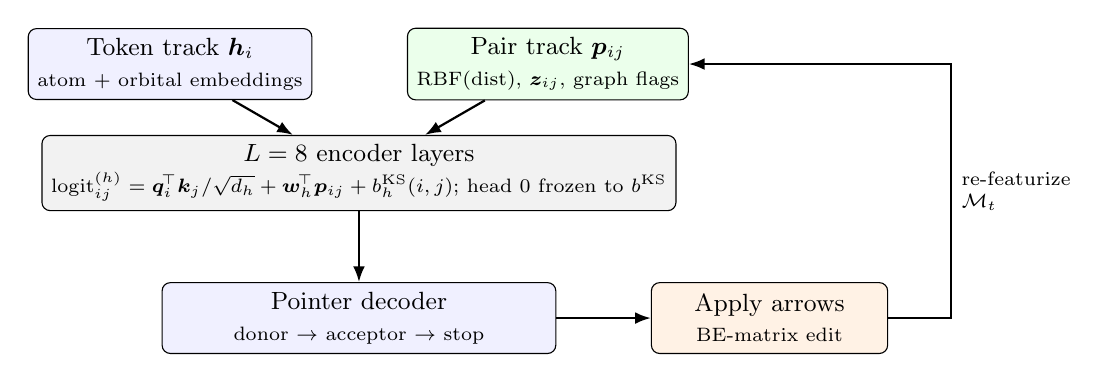
\begin{tikzpicture}[
  box/.style={draw, rounded corners=3pt, minimum height=9mm, minimum width=34mm, align=center, font=\small},
  arr/.style={-{Latex[length=2mm]}, thick},
  node distance=9mm and 12mm]
\node[box, fill=blue!6] (tok) {Token track $\vb{h}_i$\\ \scriptsize atom + orbital embeddings};
\node[box, fill=green!8, right=of tok] (pair) {Pair track $\vb{p}_{ij}$\\ \scriptsize RBF(dist), $\vb{z}_{ij}$, graph flags};
\node[box, fill=gray!10, below=of $(tok)!0.5!(pair)$, minimum width=72mm] (enc) {$L=8$ encoder layers\\ \scriptsize logit$_{ij}^{(h)}=\vb{q}_i^{\!\top}\vb{k}_j/\sqrt{d_h}+\vb{w}_h^{\!\top}\vb{p}_{ij}+b^{\KS}_h(i,j)$;\ head 0 frozen to $b^{\KS}$};
\node[box, fill=blue!6, below=of enc, minimum width=50mm] (dec) {Pointer decoder\\ \scriptsize donor $\to$ acceptor $\to$ stop};
\node[box, fill=orange!10, right=of dec, minimum width=30mm] (app) {Apply arrows\\ \scriptsize BE-matrix edit};
\draw[arr] (tok) -- (enc);
\draw[arr] (pair) -- (enc);
\draw[arr] (enc) -- (dec);
\draw[arr] (dec) -- (app);
\draw[arr] (app.east) -- ++(8mm,0) node[midway, above, font=\scriptsize, yshift=1mm, xshift=4mm]{} |- node[pos=0.25, right, font=\scriptsize, align=left]{re-featurize\\$\mathcal{M}_t$} (pair.east);
\end{tikzpicture}
\caption{Data flow for one elementary step. Both tracks are rebuilt from the re-featurized intermediate before the next step.}
\end{figure}

\subsection{Token embeddings}
\paragraph{Atom tokens.}
\begin{equation}
\begin{split}
\vb{h}^{(0)}_a={}&\vb{E}_Z[Z_a]+\vb{E}_{\mathrm{chg}}[\text{formal charge}]\\
&+\MLP_A\big([q_a,\ f^+_a,\ f^-_a,\ \Delta f_a,\ \omega_{a,\mathrm{HOMO-1..LUMO+1}},\ V^{\mathrm{bur}}_a,\ \text{chirality}]\big).
\end{split}
\end{equation}
\paragraph{Orbital tokens.}
\begin{equation}
\vb{h}^{(0)}_r=\MLP_O\big(\vb{v}^{\mathrm{cont}}_r\big)+\sum_{k}\MLP_{\Sigma}\big([\epsilon_k,\ p_{rk}]\big)+\sum_{a\in\mathcal{A}_r} w^{(r)}_a\,\vb{h}^{(0)}_a ,
\end{equation}
where $\vb{v}^{\mathrm{cont}}_r$ collects the continuous descriptors of Section~\ref{sec:tokens} (occupation, center count and weights, $s/p/d$ fractions, $\chi_a,\chi_b$, $\Pi^{(r)}_{ab}$, $R_{ab}$, $R_{\mathrm{gyr}}$), the second term is a permutation-invariant set encoder over the spectral entries, and the last term lets an orbital inherit its chemical environment from the atoms that carry it. No categorical orbital type is embedded; a unit test asserts that no model input tensor contains one. Every token also receives a fragment embedding $\vb{E}_{\mathrm{frag}}[\phi(i)\bmod 8]$, and one learned summary token $\vb{h}_{\mathrm{MECH}}$ is prepended. No absolute coordinates are embedded: geometry enters only through pairwise distances, so the model is invariant to rotations and translations by construction. Chirality is preserved through the per-atom signed-volume feature.

\subsection{Pair track initialization}
\begin{equation}
\begin{split}
\vb{p}^{(0)}_{ij}=\MLP_P\Big(\big[&\RBF(\tilde R_{ij})\odot\mathbb{1}[\phi(i)=\phi(j)],\ \vb{z}_{ij},\ \mathbb{1}[\phi(i)=\phi(j)],\\
&\mathbb{1}[\text{bonded}],\ \text{bond order},\ \min(d^{\mathrm{graph}}_{ij},6)\big]\Big),
\end{split}
\end{equation}
with $\RBF$ a bank of 32 Gaussians centred on $[0,8]$~\AA. The distance channels are masked to zero for intermolecular pairs, where the $\KS$ entries of $\vb{z}_{ij}$ already carry the contact values.

\subsection{Encoder layer}
Each of the $L=8$ layers performs, for $h=1,\dots,H-1$,
\begin{align}
\vb{q}^{(h)}_i&=\vb{W}^{(h)}_Q\LN(\vb{h}_i),\quad \vb{k}^{(h)}_j=\vb{W}^{(h)}_K\LN(\vb{h}_j),\quad \vb{v}^{(h)}_j=\vb{W}^{(h)}_V\LN(\vb{h}_j),\\
\ell^{(h)}_{ij}&=\frac{\vb{q}^{(h)\top}_i\vb{k}^{(h)}_j}{\sqrt{d_h}}
+\vb{w}_h^{\!\top}\vb{p}_{ij}
+\underbrace{\alpha_h\,\widehat{\KS}_3(i,j)+\beta_h\,\widehat{\KS}_2(i,j)-\gamma_h\,\widehat{\KS}_1(i,j)}_{b^{\KS}_h(i,j)}
+ m_{ij},
\label{eq:logit}\\
\vb{a}^{(h)}_i&=\sum_j \softmax_j\big(\ell^{(h)}_{ij}\big)\,\vb{v}^{(h)}_j ,
\end{align}
where $\widehat{\KS}$ denotes the standardized term, $\alpha_h,\beta_h,\gamma_h$ are learnable scalars initialized to $1$ and multiplied by a global scale $\lambda_{\KS}$, and $m_{ij}\in\set{0,-\infty}$ is the padding mask. The head outputs are concatenated, projected, and added residually; a position-wise feed-forward block (width $4d$, GELU) follows. The pair track is then updated in $O(N^2)$,
\begin{equation}
\vb{p}_{ij}\leftarrow\vb{p}_{ij}+\MLP_U\big([\vb{p}_{ij},\ \vb{h}_i,\ \vb{h}_j]\big),
\end{equation}
so later layers see pair features that have absorbed context from both endpoints.

\subsection{The frozen Klopman--Salem head}
Head $h=0$ has no projections and no pair weight:
\begin{equation}
\ell^{(0)}_{ij}=\widehat{\KS}_3(i,j)+\widehat{\KS}_2(i,j)-\widehat{\KS}_1(i,j)+m_{ij},\qquad
\vb{a}^{(0)}_i=\sum_j\softmax_j\big(\ell^{(0)}_{ij}\big)\,\vb{W}^{(0)}_V\LN(\vb{h}_j).
\end{equation}
Only its value projection is trained. Its attention matrix is therefore exactly the Boltzmann-like weighting that the perturbation energy prescribes, in every layer and at every stage of training. This gives (i) an ablation axis with no confound, because the physics can be removed from the other heads while head 0 is left intact or removed altogether, and (ii) an interpretation signal, because $\softmax_j(\ell^{(0)}_{ij})$ at the chosen donor $i=r$, acceptor $j=s$ states how strongly the physics alone favoured the predicted arrow. Configuration flags allow disabling all $b^{\KS}$ terms, dropping any one term, or unfreezing head 0.

\section{Pointer decoder}
\label{sec:decoder}
A step is decoded as a sequence of arrows with teacher forcing. Let $\vb{h}_i^{(L)}$ be the final token vectors and $\vb{p}^{(L)}_{ij}$ the final pair vectors.

\paragraph{Step query.}
\begin{equation}
\vb{s}_t=\MLP_S\big([\vb{h}^{(L)}_{\mathrm{MECH}},\ \vb{E}_{\mathrm{step}}[t],\ \vb{g}_{t}]\big),
\end{equation}
where $\vb{g}_t$ is the mean of the token vectors of arrows already emitted in this step (zero for the first arrow), so that concerted multi-arrow steps are decoded coherently.

\paragraph{Donor selection.} Over occupied orbital tokens with validity mask $\mathcal{V}^{\occ}$ (occupation 2, not already used in this step):
\begin{equation}
P(r\mid\cdot)=\softmax_{r\in\mathcal{V}^{\occ}}\big(\vb{s}_t^{\!\top}\vb{W}_D\,\vb{h}^{(L)}_r\big).
\end{equation}

\paragraph{Donor site.} An orbital with several centers must say on which atom the new bond forms (the terminal carbon of propene for Markovnikov addition; one of the four carbons of a ring $\pi$ orbital). Over the centers of the chosen donor, using the token-to-center incidence weights $w^{(r)}_a$:
\begin{equation}
P(a\mid r,\cdot)=\softmax_{a\in\mathcal{A}_r}\Big(\big(\vb{s}_t+\vb{h}^{(L)}_r\big)^{\!\top}\vb{W}_S\,\vb{h}^{(L)}_a+v_S\,w^{(r)}_a\Big),
\end{equation}
which is a one-entry softmax for a one-center orbital.

\paragraph{Acceptor selection.} Conditioned on the donor $r$ and its site $a$, over virtual tokens with mask $\mathcal{V}^{\virt}(r)$ (occupation 0, not the antibonding partner of the donor's own bond, no $d$-type polarization orbitals unless configured):
\begin{equation}
P(s\mid r,a,\cdot)=\softmax_{s\in\mathcal{V}^{\virt}(r)}\Big(\big(\vb{s}_t+\vb{h}^{(L)}_r+\vb{h}^{(L)}_a\big)^{\!\top}\vb{W}_A\,\vb{h}^{(L)}_s+\vb{u}^{\!\top}\vb{p}^{(L)}_{rs}\Big).
\end{equation}
The explicit pair term $\vb{u}^{\!\top}\vb{p}^{(L)}_{rs}$ is where the Klopman--Salem features of the specific candidate pair enter the arrow score directly, independently of attention.

\paragraph{Acceptor site.} Same form as the donor site, over $\mathcal{A}_s$. An arrow is therefore the 4-tuple $(r,a,s,b)$: two orbitals and the two atoms on which they meet.

\paragraph{Stop heads.} After each arrow a Bernoulli head on $[\vb{s}_t,\vb{h}_r,\vb{h}_s]$ decides \texttt{END\_STEP}; after each step a Bernoulli head on $\vb{h}^{(L)}_{\mathrm{MECH}}$ of the re-featurized intermediate decides \texttt{END\_MECH}.

\section{Training objective}
\label{sec:loss}
Dataset arrows are aligned to orbital tokens (Section~\ref{sec:align}); because several LMOs can be chemically equivalent (the two lone pairs of a carbonyl oxygen), each arrow carries label \emph{sets} $\mathcal{D}$ (donors) and $\mathcal{A}$ (acceptors). The per-arrow loss marginalizes over the sets:
\begin{equation}
\begin{split}
\mathcal{L}_{\mathrm{arrow}}={}&-\log\sum_{r\in\mathcal{D}}P(r\mid\cdot)\;-\;\log P(a^{\star}\mid r^{\star},\cdot)\\
&-\log\sum_{s\in\mathcal{A}}P(s\mid r^{\star},a^{\star},\cdot)\;-\;\log P(b^{\star}\mid s^{\star},\cdot),
\end{split}
\end{equation}
with $r^\star,s^\star$ teacher representatives of the label sets and $a^\star,b^\star$ the labeled site atoms, which are always unique because they come straight from the dataset arrow. The total loss is
\begin{equation}
\mathcal{L}=\sum_{\text{arrows}}\mathcal{L}_{\mathrm{arrow}}+\lambda_{\mathrm{stop}}\big(\mathrm{BCE}_{\texttt{END\_STEP}}+\mathrm{BCE}_{\texttt{END\_MECH}}\big),\qquad \lambda_{\mathrm{stop}}=0.5 .
\end{equation}
Each elementary step is an independent training sample; intermediates are featurized offline, so no gradient flows across steps.

\section{Label alignment and step application}

\subsection{Arrow-to-orbital alignment}
\label{sec:align}
Datasets give arrows as atom-map indices; alignment is by \emph{atom}, never by orbital label. For an arrow whose electrons leave atom $a$ (a lone pair on $a$, or a bond $(a,c)$ whose pair forms the new bond at $a$) and arrive at atom $b$ (an atom, or a bond $(b,d)$ that breaks):
\begin{itemize}[nosep]
\item donor site $a^\star=a$; $\mathcal{D}=\set{r\in\mathcal{O}^{\occ}:\ w^{(r)}_a\ge\tau_{\mathrm{atom}}}$, restricted to tokens that also have weight on $c$ for a bond source (if that empties the set the restriction is dropped and the arrow flagged);
\item acceptor site $b^\star=b$; $\mathcal{A}=\set{s\in\mathcal{O}^{\virt}:\ w^{(s)}_b\ge\tau_{\mathrm{atom}}}$, restricted to tokens with weight on $d$ for a bond sink, excluding the antibonding partner of the donor's own bond and $d$-type polarization orbitals;
\item a carbanion drawn as a lone pair on an atom that carries no one-center occupied token (an enolate in its carbanion resonance form) aligns to the multi-center tokens on that atom;
\item an empty set falls back to the tokens nearest to the atom by centroid distance and is flagged.
\end{itemize}
Sets are multi-label and the loss marginalizes over them. Because sites and sets are defined by atoms and populations, two resonance forms of the same reactant yield the same labels.

\subsection{Resonance}
\label{sec:resonance}
Products and labels are compared modulo resonance. The \emph{resonance key} of a molecule is the lexicographically smallest canonical SMILES over the RDKit resonance enumeration (capped at $1000$ structures, falling back to the plain canonical SMILES). It is used for the round-trip test, for step-level exact match, and for de-duplication. Dataset steps whose reactants and products share a key are resonance interconversions; they are removed from the training target and step indices are renumbered. Resonance structures are never enumerated as model input: the wavefunction already averages over them, and the tokens are built from it.

\subsection{Applying a step}
\label{sec:apply}
Dataset arrows are applied jointly as one edit of the bond--electron matrix (Ugi--Dugundji): a lone pair $\to$ atom creates or increments a bond and shifts formal charges $(+1,-1)$; a bond $\to$ atom decrements the bond order and shifts charges; a lone pair $\to$ bond combines the two. Predicted arrows $(r,a,s,b)$ are applied from their sites alone: form the bond $a$--$b$; if $a$ carries a negative charge or a one-center occupied token the source is treated as a lone pair, otherwise the Lewis structure is kekulized so that $a$ has a multiple bond to some $c$, that bond is decremented and the charge moved to $c$; if $s$ is an antibonding two-center token on $(b,d)$ the bond $b$--$d$ is decremented and $d$ receives the leaving charge. The result is sanitized and reduced to its resonance key. Round-trip agreement, for dataset arrows and for the labeled $(r,a,s,b)$ tuples alike, is a hard requirement of the data pipeline ($\ge95\%$ on PMechDB).

\section{Inference}
\label{sec:inference}
Given reactant SMILES: featurize (cached), encode, and run a beam search of width $B=5$ over $(r,a,s,b)$ tuples within a step, scoring by the sum of the four log-probabilities. Each completed step is applied from its sites, duplicate intermediates across beams are merged by resonance key, the intermediate is re-featurized, and decoding continues up to $T_{\max}=8$ steps or \texttt{END\_MECH}. Every returned pathway lists, per arrow, the intermediate SMILES, the step probability, the three $\KS$ values of the chosen pair, the dominant canonical MO pair $(k,m)$ in $G$ with its energies, and the frozen head's attention weight $\softmax_j(\ell^{(0)}_{rj})\big|_{j=s}$. A surrogate graph network can replace the xTB call at inference once trained on the cached records; it falls back to xTB for elements outside its training set.

\section{Complexity, invariances, and defaults}

\paragraph{Complexity.} A molecule set with $N_A$ atoms has roughly $N_O\approx 1.6\,N_A$ valence LMOs (one per bond and lone pair, plus their virtual counterparts), so $N\approx2.6\,N_A$. The pair track costs $O(N^2 d_p)$ memory per layer; for $N_A\le80$ this is below $50$~MB per sample at $d_p=64$ in mixed precision. Candidate arrows number $|\mathcal{O}^{\occ}|\cdot|\mathcal{O}^{\virt}|\le(1.3N_A)^2$.

\paragraph{Invariances.} Rotation and translation invariance hold exactly (distances only). Permutation equivariance over tokens holds by construction of attention. Mirror invariance is deliberately broken by the signed-volume chirality feature.

\begin{table}[h]
\centering
\caption{Default hyper-parameters.}
\begin{tabular}{lll}
\toprule
Symbol & Meaning & Default\\
\midrule
$d$ & token width & 256\\
$d_p$ & pair width & 64\\
$L$ & encoder layers & 8\\
$H$ & heads (incl.\ frozen head 0) & 8\\
$K$ & Wolfsberg--Helmholz constant (learnable) & init 1.75\\
$\varepsilon$ & dielectric in $\KS_2$ (learnable) & init 4.0\\
$\lambda_{\KS}$ & global scale of $b^{\KS}$ & 1.0\\
$\tau_{\mathrm{atom}}$ & population threshold for $\mathcal{A}_r$ & 0.15\\
$p_{\min}$ & spectral entry cutoff (max 8 entries) & 0.01\\
$\lambda_{\mathrm{stop}}$ & stop-loss weight & 0.5\\
$B$ & beam width & 5\\
$T_{\max}$ & max steps per mechanism & 8\\
optimizer & AdamW, lr $3\times10^{-4}$, warm-up 2k, cosine & \\
batch & 32 steps, mixed precision, grad clip 1.0 & \\
\bottomrule
\end{tabular}
\end{table}

\section{Evaluation protocol}
\begin{itemize}[nosep]
\item \textbf{Arrow level}: top-$k$ accuracy of $(r,s)$ with set marginalization ($k=1,3,5$).
\item \textbf{Step level}: exact match of the intermediate's resonance key at top-$k$.
\item \textbf{Pathway level}: full sequence recovery at beam 5; product recovered at any depth $\le8$.
\item \textbf{Validity}: sanitizable steps; conservation of heavy atoms and charge.
\item \textbf{Splits}: by reactant molecule (default, leak-proof), leave-one-mechanism-class-out, scaffold.
\item \textbf{Ablations}: no $b^{\KS}$; each term removed; head 0 unfrozen; atom-only tokens; categorical orbital labels added back as input; hybridization, aromaticity and functional-group ids added back as input (both measure what the physical descriptors already carry); $K,\varepsilon$ fixed vs.\ learned; $d$-type acceptors allowed; table vs.\ MLP contact kernel; three seeds each.
\item \textbf{Physics floor}: ranking by $\KS_3$ alone and by $\KS_3+\KS_2$ with no learned parameters; a trained model must beat it.
\item \textbf{Interpretability}: Spearman correlation between head-0 attention at the chosen pair and the model's arrow probability, per mechanism class; selectivity suite (S$_\mathrm{N}$2 vs.\ E2, 1,2- vs.\ 1,4-addition, hard/soft alkylation, Markovnikov, EAS regiochemistry, Baldwin rules).
\end{itemize}

\section{Design rationale in brief}
\begin{enumerate}[nosep]
\item \emph{Orbitals as tokens} align the prediction unit with both the arrow formalism and the perturbation theory; \emph{untyped} tokens let orbital character generalize across elements instead of being fixed by a label.
\item \emph{Pair track with physics initialization} lets the Klopman--Salem terms act as a prior on attention rather than as an auxiliary loss, so the network learns corrections to a physically shaped starting point.
\item \emph{A frozen head} makes the contribution of the physics measurable and every prediction explainable.
\item \emph{Spectral energies} make term (3) exact for localized orbitals and invariant to the arbitrary mixture a localization returns inside a flat subspace, which is what makes aromatic and conjugated systems unproblematic.
\item \emph{Contact overlaps} keep the full structure of term (3) --- exact gaps, exact coefficients --- for intermolecular steps, replacing only the one factor that no geometry can provide.
\item \emph{Sites} resolve where a multi-center orbital reacts, which is also the regiochemistry of additions to simple alkenes.
\item \emph{Deterministic step application} removes product generation from the learning problem and guarantees mass and charge conservation.
\item \emph{No chemist's taxonomy as input.} Neither orbital tokens nor atom tokens carry categorical labels ($\sigma/\pi$, hybridization, aromaticity, functional group); everything the model sees is a physical quantity or a Lewis-bookkeeping integer. The one deliberate prior is the frozen Klopman--Salem head, which is declared, measurable and removable.
\end{enumerate}

\end{document}
